%%%%%%%%%%%%%%%%%%%%%%%%%%%%%%%%%%%%%%%%%
% The Legrand Orange Book
% LaTeX Template
% Version 2.1.1 (14/2/16)
%
% This template has been downloaded from:
% http://www.LaTeXTemplates.com
%
% Original author:
% Mathias Legrand (legrand.mathias@gmail.com) with modifications by:
% Vel (vel@latextemplates.com)
%
% License:
% CC BY-NC-SA 3.0 (http://creativecommons.org/licenses/by-nc-sa/3.0/)
%
% Compiling this template:
% This template uses biber for its bibliography and makeindex for its index.
% When you first open the template, compile it from the command line with the 
% commands below to make sure your LaTeX distribution is configured correctly:
%
% 1) pdflatex main
% 2) makeindex main.idx -s StyleInd.ist
% 3) biber main
% 4) pdflatex main x 2
%
% After this, when you wish to update the bibliography/index use the appropriate
% command above and make sure to compile with pdflatex several times 
% afterwards to propagate your changes to the document.
%
% This template also uses a number of packages which may need to be
% updated to the newest versions for the template to compile. It is strongly
% recommended you update your LaTeX distribution if you have any
% compilation errors.
%
% Important note:
% Chapter heading images should have a 2:1 width:height ratio,
% e.g. 920px width and 460px height.
%
%%%%%%%%%%%%%%%%%%%%%%%%%%%%%%%%%%%%%%%%%

%----------------------------------------------------------------------------------------
%	PACKAGES AND OTHER DOCUMENT CONFIGURATIONS
%----------------------------------------------------------------------------------------

\documentclass[11pt,fleqn]{book} % Default font size and left-justified equations

\usepackage{wasysym}
\usepackage{esint} % various fancy integral symbols
\usepackage{tikz}
\usepackage{tikz-3dplot}
\usepackage{pgfplots}
\pgfplotsset{compat=1.17}
\usetikzlibrary{patterns}
\usepackage{tkz-euclide} 
\usepackage{mathtools}
\usepackage{xurl}
\usepackage[version=4,arrows=pgf-filled,
textfontname=sffamily,
mathfontname=mathsf]{mhchem}
\usepackage{gensymb}
\usepackage{tabularray}

\usetikzlibrary {arrows.meta} 

\newcommand{\degC}{{\degree}C}
\newcommand{\dd}{\mathrm{d}}
\newcommand{\div}{\mathrm{div}}
\newcommand{\rot}{\vv{\mathrm{div}}}
\newcommand{\grad}{\vv{\mathrm{grad}}}

\tikzset{
    support/.style={
        pattern=north east lines,
        draw=none,
        minimum width=0.3,
        minimum height=0.6
    }
    ,>=latex
}

\usepackage[d]{esvect}

%SPECIFIC TO THIS CHAPTER
\usepackage{physics}
\usepackage{ifthen}
\usepackage[outline]{contour} % glow around text
\usetikzlibrary{calc} % for pic
\usetikzlibrary{angles,quotes} % for pic
\usetikzlibrary{patterns}
\tikzset{>=latex} % for LaTeX arrow head
\contourlength{1.2pt}

\colorlet{myred}{red!65!black}
\definecolor{myred}{RGB}{255,81,46}
\tikzstyle{ground}=[preaction={fill,top color=black!10,bottom color=black!5,shading angle=20},
                    fill,pattern=north east lines,draw=none,minimum width=0.3,minimum height=0.6]
\tikzstyle{mass}=[line width=0.6,myred,fill=myred!40,rounded corners=1,
                  top color=myred!40,bottom color=myred!20,shading angle=20]
\tikzstyle{rope}=[myred!30,line width=1.2,line cap=round] %very thick

% FORCES SWITCH
\tikzstyle{force}=[->,myred,ultra thick,line cap=round]
\tikzstyle{Fproj}=[force,myred!60]
\newboolean{showforces}
\setboolean{showforces}{true}
%----------------------------------------------------------------------------------------

\input{structure} % Insert the commands.tex file which contains the majority of the structure behind the template

\begin{document}

%----------------------------------------------------------------------------------------
%	TABLE OF CONTENTS
%----------------------------------------------------------------------------------------

%\usechapterimagefalse % If you don't want to include a chapter image, use this to toggle images off - it can be enabled later with \usechapterimagetrue

\chapterimage{cellule_diamant_schema.png} % Table of contents heading image

%\pagestyle{empty} % No headers

%\tableofcontents % Print the table of contents itself

%\cleardoublepage % Forces the first chapter to start on an odd page so it's on the right

%\pagestyle{fancy} % Print headers again



%\part{\'{E}lectromagnétisme}

\setcounter{chapter}{5}

\chapter{Optimisation d'un procédé chimique}

\section{Notion d'équilibre chimique}

Les réactions chimiques sont omniprésentes dans l'industrie aujourd'hui, que ce soit pour produire de l'énergie thermique ou électrique, ou pour synthétiser des composés.

Pour savoir si une réaction chimique peut effectivement avoir lieu ou non, et si cela est efficace, vous avez vu en première année la constante d'équilibre, qui caractérise une réaction. Dans ce chapitre, nous allons essayer de caractériser l'évolution et l'équilibre d'un système chimique de façon plus rigoureuse, avec les outils de la thermodynamique, qui nous permettront de démontrer la loi d'actions de masse.

Pour cela, nous considérons une réaction chimique monotherme et monobare, c'est-à-dire que la température extérieure et la pression extérieure sont constantes. Nous supposons que les réactifs et les produits restent dans un réacteur chimique qui correspond à notre système $\Sigma$. Le système subit une transformation chimique entre deux états d'équilibre. Nous appliquons le second principe de la thermodynamique, dont on rappelle ici l'expression :
\begin{theorem}
    Soit $\Sigma$ un système physico-chimique fermé. La variation d'entropie du système au cours d'une transformation thermodynamique est donnée par :
    \begin{equation}
        \Delta S = S_{créée} + S_{échangée}
    \end{equation}
    où l'entropie créée au cours de la transformation est toujours positive, et l'entropie échangée est :
    \begin{equation}
        S_{échangée} = \int \frac{\delta Q}{T_{ext}}
    \end{equation}
    avec $Q$ l'énergie thermique reçue par $\Sigma$ au cours de la transformation, et $T_{ext}$ la température extérieure.
\end{theorem}
Ici, la transformation étant monotherme, l'intégrale se simplifie et on peut écrire $S_{échangée} = Q/T_{ext}$. On en déduit qu'au cours de la transformation :
\begin{equation}
    \Delta S - \frac{Q}{T_{ext}} > 0
\end{equation}
Or, puisque la transformation est monobare, nous pouvons utiliser la relation suivante que nous avons démontrée dans le chapitre précédent :
\begin{equation}
    Q = \Delta H
\end{equation}
où $H$ est l'enthalpie du système. On obtient ainsi :
\begin{equation}
    \Delta H = T_{ext} \Delta S < 0
\end{equation}
Comme la transformation se fait entre deux états d'équilibre, nous avons $T_{initiale} = T_{finale} = T_{ext}$ et nous pouvons conclure que :
\begin{equation}
    \Delta(H - TS) < 0
\end{equation}
La quantité $H - TS$ ne peut que décroître au cours de la transformation : on dit que c'est un potentiel thermodynamique. C'est une conséquence directe du second principe. Cette équation nous informe sur le sens d'évolution d'une réaction chimique : la réaction va avoir lieu dans le sens qui a tendance à diminuer cette quantité. On définit donc l'enthalpie libre d'un système :
\begin{definition}
    L'enthalpie libre $G$ d'un système thermodynamique $\Sigma$ est définie en fonction de son énergie interne $U$, sa pression $p$, son volume $V$, sa température $T$ et son entropie $S$:
    \begin{equation}
        G = U + pV - TS
    \end{equation}
    Elle peut ausi s'écrire en fonction de l'enthalpie $H$:
    \begin{equation}
        G = H -TS
    \end{equation}
\end{definition}

\begin{proposition}
    Si un système fermé subit une transformation thermodynamique monotherme et monobare, alors son enthalpie libre ne peut que diminuer.
\end{proposition}

Nous avons donc démontrer que le système chimique va évoluer dans le sens qui minimise son enthalpie libre. En particulier, l'avancement de la réaction $\xi$ va évoluer de sorte à ce qu'il minimise l'enthalpie libre. Nous pouvons alors définir l'enthalpie libre de réaction, de la même manière que nous avons défini l'enthalpie de réaction :
\begin{definition}
    L'enthalpie libre d'une réaction chimique, notée $\Delta_r G$, correspond à la variation d'enthalpie d'un système chimique par unité d'avancement au cours d'une transformation monotherme et monobare. Autrement dit :
    \begin{equation}
        \Delta_r G(T,p,\xi) = \left. \frac{\partial G}{\partial \xi} \right|_{T,p}
    \end{equation}
\end{definition}

Si $\Delta_r G <0$, alors la réaction évolue dans le sens direct. Au contraire, si $\Delta_r G > 0$, la réaction évolue dans le sens inverse. L'équilibre est atteint lorsque l'enthalpie est minimale, c'est-à-dire lorsque $\Delta_r G = 0$, comme on peut le voir sur la figure \ref{fig:enthalpie_libre_reaction}.

\begin{figure}[htbp]
    \centering
    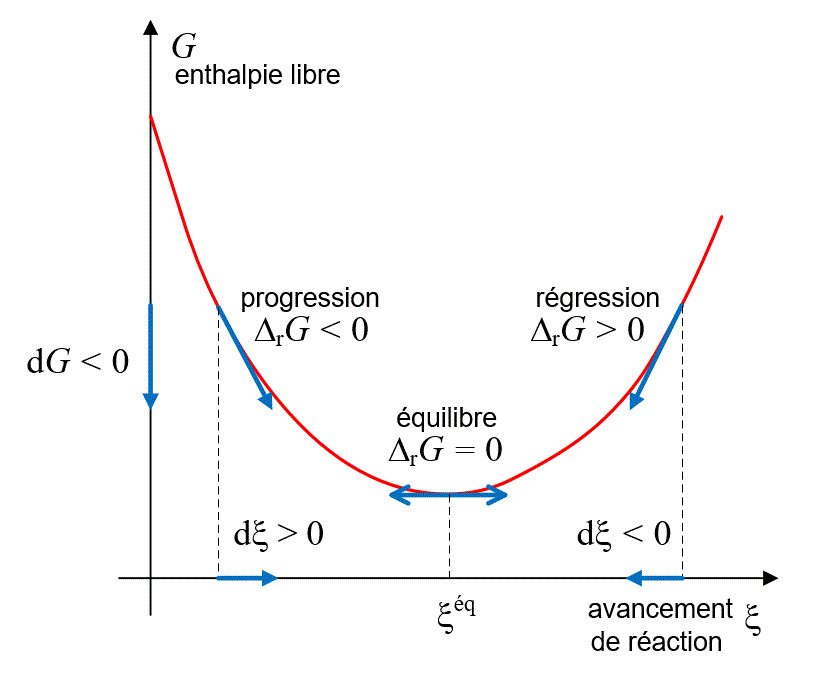
\includegraphics[width=0.7\linewidth]{Pictures/deplacement_equilibre.jpg}
    \caption{Enthalpie libre du système $G$ en fonction de l'avancement. L'enthalpie libre de réaction correspond à la pente de la courbe. L'état d'équilibre est atteint lorsque l'enthalpie est minimale, et l'enthalpie libre de réaction est nulle. Source : Wikimedia Commons.}
    \label{fig:enthalpie_libre_reaction}
\end{figure}

A priori, l'enthalpie libre de réaction dépend de l'avancement de la réaction et plus généralement des concentrations ou pressions partielles des constituants chimiques du mélange. Il n'est donc pas possible de la tabuler directement. Pour cela, nous définissons l'enthalpie libre standard de réaction :
\begin{definition}
    L'enthalpie libre standard d'une réaction chimique, notée $\Delta_r G\degree(T)$, est l'enthalpie libre de la réaction lorsque les constituants sont tous pris dans leur état standard.
\end{definition}
\begin{remark}
    Puisque les constituants sont pris dans leur état standard, leur concentration/pression partielle est fixe et l'enthalpie libre standard de réaction ne dépend donc que de la température.
\end{remark}

En général, l'enthalpie libre standard de réaction nous informe si une réaction chimique va se faire spontanément ou non dans les conditions usuelles de pression et de température. Si $\Delta_rG\degree<0$ la réaction aura tendance à se faire spontanément, sinon il sera nécessaire de jouer sur les paramètres extérieurs pour favoriser la réaction: c'est ce que l'on appelle l'optimisation chimique. Pour pouvoir prévoir le caractère spontané ou non de la réaction, il est donc nécessaire de mieux caractériser l'enthalpie libre standard de réaction, afin de comprendre ce qui fixe l'équilibre chimique et comment l'optimiser.

\section{Potentiel chimique}

Pour cela, nous pouvons noter $n_i$ la quantité de matière de chaque constituant $A_i$ dans le système physico-chimique, et nous appelons $\nu_i$ le coefficient stoechiométrique algébrique associé dans la réaction, qui peut s'écrire :
\begin{equation}
    \sum_i \nu_i A_i = 0
\end{equation}

L'enthalpie libre du système dépend a priori de la température, de la pression, et des quantités de matière de chaque constituant :
\begin{equation}
    G = G(T,p, n_1, ..., n_N)
\end{equation}
Nous définissons le potentiel chimique $\mu_i$ d'un constituant de la façon suivante :
\begin{definition}
    \begin{equation}
    \mu_i = \left. \frac{\partial G}{\partial n_i} \right|_{T,p}
    \end{equation}
    Il mesure la variation d'enthalpie libre produite par l'introduction d'une mole de ce constituant.
\end{definition}

Ce potentiel chimique est utile, car l'enthalpie libre de réaction s'écrit comme une combinaison linéaire des potentiels chimiques :
\begin{theorem}
    Soit une réaction chimique faisant intervenir les constituants $A_i$ qui s'écrit de façon algébrique :
    \begin{equation}
    \sum_i \nu_i A_i = 0
\end{equation}
Alors l'enthalpie libre $\Delta_r G$ de la réaction est fonction des potentiels chimiques $\mu_i$ des constituants :
\begin{equation}
    \Delta_r G = \sum_i \nu_i \mu_i
\end{equation}
\end{theorem}

\begin{demonstration}
    Pour le démontrer, nous utilisons le fait que l'enthalpie libre est une grandeur extensive. Ainsi, si on multiplie toutes les quantités de matière par une constante $\lambda$, on doit également multiplier $G$ par $\lambda$ :
    \begin{equation}
        G(T,p,\lambda n_1,...,\lambda n_N) = \lambda G(T,p,n_1,...,n_N)
    \end{equation}
    On dérive par rapport à $\lambda$ :
    \begin{equation}
        \sum_i \left. \frac{\partial G}{\partial n_i} \right|_{T,p} n_i = G
    \end{equation}
    ou encore en utilisant la définition du potentiel chimique :
    \begin{equation}
        G = \sum_i \mu_i n_i
    \end{equation}
    Enfin, au cours de la réaction, les quantités de matière varient en fonction de l'avancement :
    \begin{equation}
        \dd n_i = \nu_i \dd \xi
    \end{equation}
    si bien que l'on peut écrire :
    \begin{equation}
        \frac{\partial G}{\partial \xi} = \sum_i \mu_i \nu_i
    \end{equation}
    En utilisant la définition de l'enthalpie libre de réaction, on obtient bien le résultat à prouver.
\end{demonstration}

Nous avons maintenant avancé : nous avons montré que le sens de la réaction est dicté par l'enthalpie libre de réaction, et que celle-ci dépend des potentiels chimiques des constituants du mélange.

\subsection{Expression des potentiels chimiques}

Nous admettons que les potentiels chimiques d'une espèce s'écrivent de la forme suivante :
\begin{proposition}
    Soit un constituant $A_i$ dont l'activité est notée $a_i$. Alors le potentiel chimique de ce constituant s'écrit :
    \begin{equation}
        \mu_i = \mu_i\degree(T) + RT \ln(a_i)
    \end{equation}
    où $R$ est la constante des gaz parfaits, $T$ est la température et $\mu_i\degree(T)$ est le potentiel chimique standard de l'espèce à la température $T$.
\end{proposition}
\begin{remark}
    Cette expression peut se démontrer à partir de lois de la thermodynamique, en particulier pour les gaz parfaits, mais la démonstration n'est pas au programme de MP.
\end{remark}

Nous rappelons ici les expressions des activités des différents constituants en fonction de leur phase :
\begin{proposition}[Activité d'un gaz parfait]
    Si $A_i$ est un gaz parfait de pression partielle $p_i$ situé dans un mélange de gaz parfaits, son activité est :
    \begin{equation}
        a_i = \frac{p_i}{P\degree}
    \end{equation}
    où $P\degree$ est la pression standard.
\end{proposition}
\begin{proposition}[Activité d'un soluté]
    Si $A_i$ est en solution, en négligeant les interactions entre différentes molécules/ions de soluté, son activité est :
    \begin{equation}
        a_i = \frac{[A_i]}{c\degree}
    \end{equation}
    où $c\degree$ est la concentration standard.
\end{proposition}
\begin{proposition}[Activité d'un solvant ou d'une phase condensée]
    Si $A_i$ est un solvant ou une phase condensée son activité est approximativement égale à 1 :
    \begin{equation}
        a_i \approx 1
    \end{equation}
\end{proposition}

Nous obtenons alors l'expression suivante de l'enthalpie libre de réaction :
\begin{equation}
    \Delta_r G = \sum_i \nu_i\left(\mu_i\degree(T) + RT \ln(a_i)\right)
\end{equation}
Nous remarquons que lorsque les constituants sont tous dans leur état standard, leur activité est égale à 1, si bien que le second terme dans la somme est nulle. Nous avons donc la relation suivante :
\begin{proposition}
    L'enthalpie libre standard de réaction s'exprime en fonction des potentiels chimiques standard :
    \begin{equation}
        \Delta_r G\degree = \sum_i \nu_i \mu_i\degree
    \end{equation}
\end{proposition}

Rappelons-nous maintenant de la définition du quotient de réaction, vue en première année :
\begin{definition}
    Le quotient de réaction $Q$ d'une réaction de la forme $\sum_i \nu_i A_i =0$ est défini en fonction des activités $a_i$ des différents constituants :
    \begin{equation}
        Q = \prod_i a_i^{\nu_i}
    \end{equation}
\end{definition}
Nous pouvons alors remarquer que, en raison des propriétés du logarithme :
\begin{equation}
    \ln Q = \sum_i \nu_i \ln a_i
\end{equation}

Ainsi, l'expression de l'enthalpie libre standard de réaction est directement liée au quotient réactionnel :
\begin{proposition}
    L'enthalpie libre d'une réaction chimique s'exprime en fonction du quotient réactionnel et de l'enthalpie libre standard :
    \begin{equation}
        \Delta_r G = \Delta_r G\degree + RT \ln(Q)
    \end{equation}
\end{proposition}

A l'équilibre chimique, l'enthalpie libre de réaction est nulle. Ainsi, nous retrouvons la loi d'actions de masse :
\begin{theorem}[Loi d'actions de masse]
    A l'équilibre chimique, le quotient réactionnel est relié à l'enthalpie libre de réaction par la relation suivante :
    \begin{equation}
        Q = \exp \left( - \frac{\Delta_rG\degree}{RT} \right) = K\degree(T)
    \end{equation}
    où l'on a défini la constante de réaction $K\degree(T)$ qui ne dépend que de la température.
\end{theorem}
\begin{remark}
    La loi d'actions de masse caractérise l'équilibre d'un système chimique. Elle nous permet de savoir comment un système va évoluer lorsque l'on fait varier les activités des constituants chimiques du mélange ou les paramètres extérieurs (pression, température). Elle est essentielle pour pouvoir prédire l'efficacité d'une réaction chimique et son avancement final. Dans ce chapitre, nous avons pu démontrer que la loi d'actions de masse est une conséquence du second principe de la thermodynamique, et qu'elle traduit la minimisation d'un potentiel thermodynamique : l'enthalpie libre.
\end{remark}

De manière plus générale, il existe une relation directe entre enthalpie libre de réaction et quotient de réaction :
\begin{proposition}
    L'enthalpie libre de réaction dépend du quotient de réaction et de la constante d'équilibre de la réaction :
    \begin{equation}
        \Delta_r G = R T \ln \left( \frac{Q}{K\degree(T)} \right)
    \end{equation}
    Ainsi, si $Q < K\degree(T)$, $\Delta_rG<0$ et la réaction évolue dans le sens direct. Si $Q > K\degree(T)$, $\Delta_rG>0$ et la réaction évolue dans le sens indirect. 
\end{proposition}

\section{Méthodes d'optimisation}

Nous allons maintenant nous intéresser aux différentes méthode d'optimisation. Elles se basent sur différentes propriétés de l'enthalpie libre de réaction, mais on constate empiriquement qu'elles obéissent toujours au principe de La Châtelier :
\begin{theorem}
    Lorsque l'on perturbe les conditions d'un système réactif à l'équilibre, l'équilibre va spontanément être déplacé dans le sens qui tend à s'opposer à la perturbation imposée.
\end{theorem}
\begin{remark}
    Cette loi est une loi empirique. Elle n'est pas au programme, veillez donc à ne pas l'utiliser en concours pour justifier votre raisonnement. Mais vous pouvez vous en servir à l'oral, ou bien pour vous-même pour vérifier la cohérence de vos résultats.
\end{remark}

La relation à l'équilibre s'écrit :
\begin{equation}
    \prod_i a_i^{\nu_i} = K\degree(T)
\end{equation}
Les activités peuvent être écrites en fonction des conditions environnementales et des quantités initiales de réactifs. En agissant sur ces grandeurs, on va pouvoir modifier la solution de l'équation et maximiser l'avancement, donc le rendement de la réaction.

Nous allons nous intéresser en particulier à une expérience illustrative que nous pouvons faire en classe :
\begin{equation}
    \ce{\color{blue}{[Cu(H2O)6]^{2+}(aq)} + 4 Cl-(aq) = \color{green}{[CuCl4]^{2-}(aq)} + 6H2O(l)}
\end{equation}
Les procédés d'optimisation, bien sûr, s'appliquent en général à des réactions faites dans le milieu de l'industrie, pour lesquelles les problématiques de rendement sont très importantes. On peut citer notamment la réaction de production de l'ammoniaque, un fort engrais, ou encore les questions de stockage de l'hydrogène.

\begin{figure}[htbp]
    \centering
    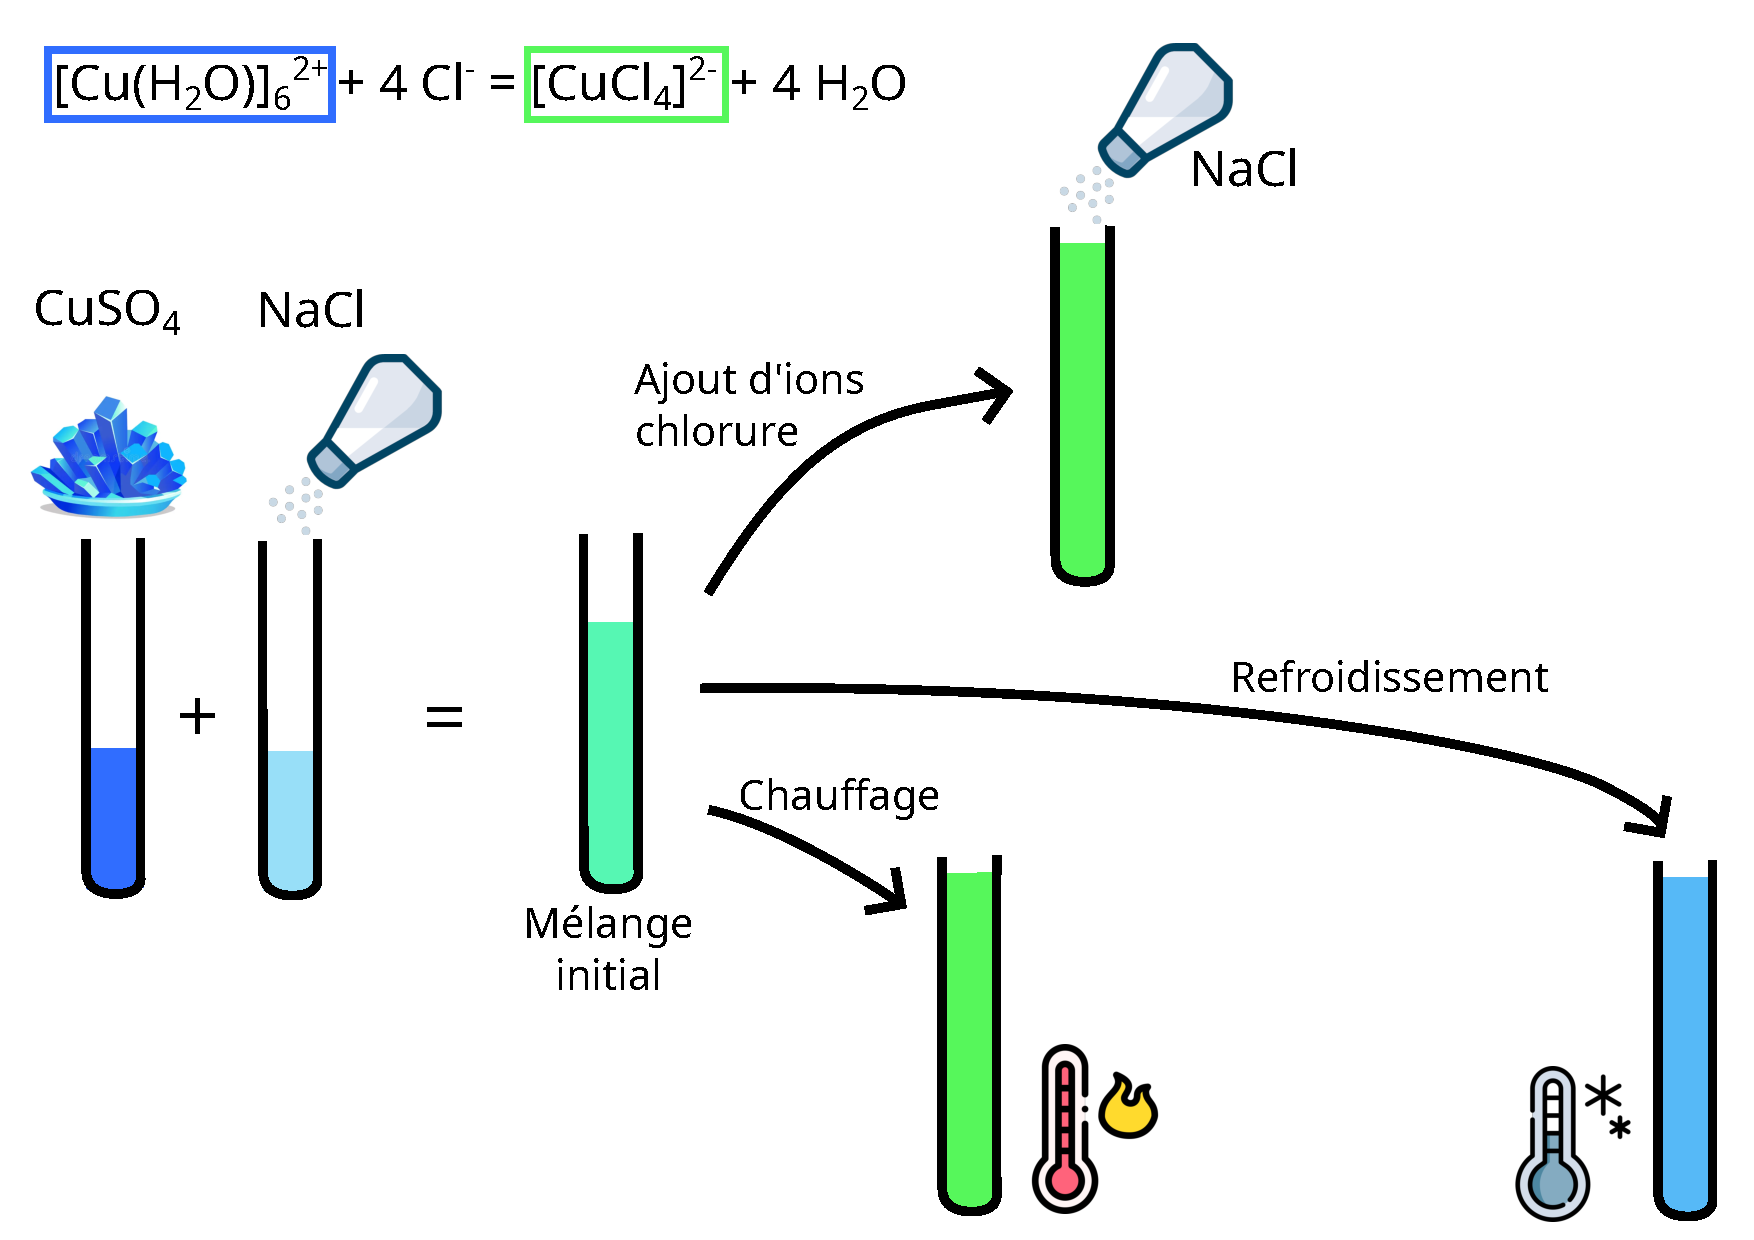
\includegraphics[width=\linewidth]{Pictures/reaction_so4cl.pdf}
    \caption{Synthèse des résultats expérimentaux obtenus en faisant réagir des ions cuivre (II) (bleus) avec des ions chlorure incolores. Le produit de la réaction, le tétrachlorure de cuivre (II), est vert. On constate un déplacement d'équilibre lorsque l'on introduit du réactif limitant en excès, ou si l'on modifie la température sans ajouter ni retirer de réactifs.}
    \label{fig:reaction_so4cl}
\end{figure}

 \subsection{Modification de la stoechiométrie}

 Une première façon de modifier l'avancement est d'augmenter l'activité de certains réactifs. En effet, les réactifs étant au dénominateur de $Q$, en augmentant leur activité, on diminue $Q$ et on favorise un déplacement de l'équilibre dans le sens direct. Ceci peut être atteint en introduisant l'un des réactifs \textbf{non limitants} en large excès. Par exemple, dans notre cas, nous pouvons ajouter en large excès du sel (chlorure de sodium), qui est peu cher et peu polluant. Cela va contribuer à augmenter l'avancement alors que la quantité de réactif limitant ne change pas, et donc augmenter le rendement.
 \begin{remark}
    Attention ! Si l'on augmente la quantité de \textbf{tous} les réactifs, on va évidemment diminuer $Q$ et faire évoluer la réaction dans le sens direct, mais on n'améliorera pas forcément le rendement. En effet, le rendement est calculé en fonction du réactif limitant. Si on augmente l'activité du réactif limitant, on augmente l'avancement de la réaction mais pas forcément le rendement.
 \end{remark}

 Pour s'en convaincre, on dresse le tableau d'avancement suivant. On choisit un tableau en concentrations :

 
 \begin{tblr}{%
  vlines, hlines,
  colspec = {Q[c] Q[c] X[c] X[c] X[c] X[c]},
  vline{4} = {1}{ text = \clap{\ce{+}} },
  vline{5} = {1}{ text = \clap{\ce{->}} },
  vline{6} = {1}{ text = \clap{\ce{+}} },
}
  État          & Avancement & \ce{[Cu(H2O)6]^{2+}}   & \ce{4 Cl-}   & \ce{6 H2O} & \ce{[CuCl4]^{2-}}  \\
  Initial       & $x=0$      & $c_1$      & $c_2$       & excès        & 0 \\
  Intermédiaire & $x$        & $c_1-x$    & $c_2-4x$    & excès      & $x$ \\
  Final         & $\xi_f$      & $c_1-x_f$  & $c_2-4x_f$  & excès   & $x_f$ \\
\end{tblr}


Le quotient de réaction s'écrit alors, à l'équilibre :
\begin{equation}
    Q = \frac{x_f c\degree^4}{(c_1-x_f)(c_2-4x_f)^4} = K\degree(T)
\end{equation}
Supposons que le réactif limitant est le cuivre hydraté. Alors le rendement de la réaction est donné par $\eta = x_f/c_1$ et l'on peut écrire :
\begin{equation}
    Q = \frac{\eta}{(1-\eta)\left(\frac{c_2}{c_1}-4\eta\right)^4} \cdot \left( \frac{c\degree}{c_1}\right)^4 = K\degree(T)
\end{equation}
Si on augmente $c_2/c_1$, alors on diminue le quotient de réaction et on fait augmenter le rendement de la réaction. On constate donc que pour optimiser le rendement on peut introduire l'un des réactifs en large excès.

Cette méthode est compatible avec le principe de modération de La Châtelier : si on introduit un réactif en excès, la réaction va évoluer dans le sens de la consommation de ce réactif.

Cette méthode fonctionne bien si l'un des réactifs est beaucoup plus cher que l'autre et s'il n'est pas polluant.

\subsection{Modification de la pression}

Dans le cadre d'une réaction chimique impliquant des composés gazeux, on peut également agir sur la pression. Nous pouvons prendre l'exemple de la réaction de formation de l'hydrure de palladium, un métal qui permet de stocker de l'hydrogène sous une forme moins volumineuse :
\begin{equation}
    \ce{2 Pd(s) + H2(g) = 2 PdH(s)}
\end{equation}
Les composés solides ayant une activité de 1, le quotient réactionnel s'écrit :
\begin{equation}
    Q = \frac{p\degree}{p_{\ce{H2}}} = \frac{p\degree}{p\, x_{\ce{H2}}}
\end{equation}
où $x_{\ce{H2}}$ est la fraction molaire en dihydrogène. En augmentant la pression totale, on augmente ainsi la pression partielle en dihydrogène et on réduit le quotient réactionnel, ce qui fait évoluer la réaction dans le sens direct. Ceci est compatible avec le principe de Le Châtelier : une augmentation de la pression fait évoluer le système dans le sens de la consommation du gaz.

De manière générale, on a la propriété suivante :
\begin{proposition}
    Une augmentation de la pression déplace l'équilibre dans le sens qui fait diminuer le nombre de moles de gaz.
\end{proposition}
\begin{demonstration}
    Cette démonstration formelle n'est pas à connaître. Par contre, il faut savoir mener ce raisonnement pour un exemple (cf TD). Considérons une réaction de la forme :
    \begin{equation}
        \sum_i \nu_i A_i + \sum_j \nu_j' G_j
    \end{equation}
    où les composés $G_j$ sont gazeux et les autres sont non gazeux. Nous notons $p$ la pression totale et $x_j$ la fraction molaire de chacun des composés. Le quotient réactionnel s'écrit alors :
    \begin{equation}
        Q = \prod_i a_i^{\nu_i} \times \prod_j \left( \frac{x_j p}{P\degree}\right)^{\nu_j'} = \prod_i a_i^{\nu_i} \times \prod_j x_j^{\nu_j'} \times \left( \frac{p}{P\degree} \right)^{\sum_j \nu_j'}
    \end{equation}
    En isolant le dernier facteur, on constate que la dépendance de $Q$ à la pression totale $p$ dépend de la somme $\sum_j \nu_j'$ :
    \begin{itemize}
        \item Si $\sum_j \nu_j'<0$, la réaction diminue le nombre de moles de gaz dans le sens direct. Une augmentation de la pression fait diminuer $Q$, et la réaction évolue dans le sens direct.
        \item Si $\sum_j \nu_j'>0$, la réaction augmente le nombre de moles de gaz dans le sens direct. Une augmentation de la pression fait augmenter $Q$, et la réaction évolue dans le sens indirect.
    \end{itemize}
    L'augmentation de la pression fait donc évoluer l'aquilibre dans le sens d'une diminution du nombre de moles de gaz, ce qui est cohérent avec le principe de modération de La Châtelier.
\end{demonstration}

\begin{encart}[Stockage de l'hydrogène]
    L'hydrogène est souvent présenté comme un carburant vert en raison de nombreux avantages : il peut être produit à partir d'électricité, et donc directement des énergies renouvelables. Sa combustion, par ailleurs, ne produit pas de dioxyde de carbone et ne contribue donc pas au réchauffement climatique.

    L'inconvénient majeur de l'hydrogène est son stockage : sa température d'ébullition est de 20\,K ce qui empêche de le stocker sous forme liquide, et en raison de sa très faible masse molaire ($M = 1$\,g$\cdot$mol$^{-1}$), il est très volumineux à la forme gazeuse. Des recherches sont en cours pour trouver un moyen de le stocker de manière moins encombrante.

    L'une des méthodes envisagées est la production d'hydrures de métaux : ce sont des solides cristallins dans lesquels s'insèrent des atomes d'hydrogène. L'hydrure de palladium est l'une des solutions envisagées. Pour le synthétiser, on utilise des cellules à enclumes de diamant, qui permettent d'augmenter fortement la pression sur l'échantillon en appliquant une force donnée sur une surface très faible d'échantillon. La pression peut atteindre 30\,000 bars. Augmenter la pression dans l'échantillon permet de favoriser la formation de l'hydrure, comme nous l'avons vu plus haut. Ainsi, il est possible de produire de l'hydrure de palladium même si la constante de réaction est très faible, en jouant sur les conditions environnementales.

    \begin{center}
        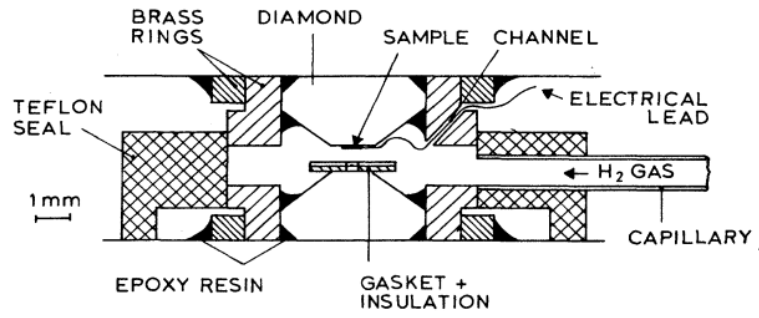
\includegraphics[width=0.6\linewidth]{Pictures/fabrication_PdH.png} \\
        Synthèse de l'hydrure de palladium dans une cellule à enclumes de diamant. Source : Hemmes et al (1989).
    \end{center}
\end{encart}

\subsection{Influence de la température}

Nous pouvons finalement nous intéresser à la température. Celle-ci n'agit pas sur les activités des constituants chimiques, donc pas sur le quotient de réaction, mais elle agit directement sur la constante de réaction $K\degree(T)$.

Nous pouvons prendre l'exemple de la réaction de formation du tétrachlorure de cuivre :
\begin{equation}
    \ce{\color{blue}{[Cu(H2O)6]^{2+}(aq)} + 4 Cl-(aq) = \color{green}{[CuCl4]^{2-}(aq)} + 6H2O(l)}
\end{equation}
On constate qu'en augmentant la température, l'équilibre est déplacé dans le sens direct, alors qu'en diminuant la température, il est déplacé dans le sens inverse. Cela signifie que la constante de réaction $K\degree(T)$ augmente avec la température.

La dépendance de cette constante en fonction de la température est donnée par la relation de Van't Hoff :
\begin{theorem}[Loi de Van't Hoff]
    La constante d'équilibre $K\degree(T)$ d'une réaction chimique dépend de la température selon la loi suivante :
    \begin{equation}
        \frac{\dd \ln K\degree}{\dd T} = \frac{\Delta_r H\degree}{R T²}
    \end{equation}
    où $\Delta_r H\degree$ est l'enthalpie standard de réaction, et $R$ la constante des gaz parfaits. 
\end{theorem}
\begin{demonstration}
    Par définition de la constante de réaction :
    \begin{equation}
        \ln K\degree  = - \frac{\Delta_r G\degree}{RT}
    \end{equation}
    On dérive par rapport à la température :
    \begin{equation}
        \frac{\dd \ln K\degree}{\dd T} = \frac{\Delta_r G\degree}{RT^2} - \frac{1}{RT} \frac{\dd \Delta_r G\degree}{\dd T}
    \end{equation}
    Or, on a vu que $G = H - TS$. La transformation chimique étant supposée monotherme entre deux états d'équilibre, on en déduit que $T_{initiale} = T_{finale} = T_{ext}$ et au cours de la transformation : $\Delta G = \Delta H - T \Delta S$. Ainsi, en appliquant cette relation aux conditions standard :
    \begin{equation}
        \Delta_r G\degree = \Delta_r H\degree - T \Delta_r S\degree
    \end{equation}
    où l'entropie standard de réaction est définie de la même façon que les enthalpies et enthalpies libres standard de réaction : la variation d'entropie par unité d'avancement pour une réaction dans les conditions standard. On obtient alors :
    \begin{equation}
        \frac{\dd \Delta_r G\degree}{\dd T} = - \Delta_r S\degree
    \end{equation}
    Si bien que :
    \begin{equation}
    \frac{\dd \ln K\degree}{\dd T} = \frac{\Delta_r G\degree}{RT^2} + \frac{\Delta_r S\degree}{RT} = \frac{\Delta_r H\degree}{R T^2}
    \end{equation}
    (on a utilisé à nouveau la relation $\Delta_rG\degree = \Delta_rH\degree-T\Delta_rS\degree$). On obtient bien la loi de Van't Hoff.
\end{demonstration}

On peut vérifier la compatibilité de la loi de Van't Hoff avec le principe de modération de La Châtelier. Si la réaction est endothermique, alors $\Delta_r H\degree > 0$. Lorsque la température augmente, d'après la loi de Van't Hoff, la constante d'équilibre va augmenter et l'équilibre évolue dans le sens direct, c'est-à-dire qu'il consomme de l'énergie thermique, ce qui vient s'oppposer à la diminution initiale de la température.

Au contraire, si la réaction est exothermique, une augmentation de la température fait évoluer l'équilibre dans le sens indirect, ce qui consomme de l'énergie thermique et s'oppose également à la diminution initiale de température.

Dans le cadre de notre expérience avec le cuivre, nous avons observé un déplacement de l'équilibre dans le sens direct lors d'une augmentation de température, ce qui semble indiquer que la réaction se fait dans le sens direct. Pour le vérifier, nous pouvons refaire la réaction avec un thermomètre : nous constatons effectivement que la réaction est endothermique.

\section{Loi de Hess et calcul de l'enthalpie libre standard de réaction}

De la même manière que l'enthalpie standard de réaction, l'enthalpie libre standard de réaction ne peut pas être tabulée pour toutes les réactions chimiques possibles. Pour la calculer, nous utilisons également la loi de Hess.

Nous avons rapidement défini, lors de la démonstration de la loi de Van't Hoff, une entropie standard de réaction. Pour définir plus rigoureusement cette quantité nous pouvons définir l'entropie standard d'un constituant :
\begin{definition}
    L'entropie standard $S\degree$ d'un constituant chimique est son entropie par unité de quantité de matière, lorsqu'il est dans son état standard. C'est une grandeur intensive qui se mesure en J$\cdot$K$^{-1}\cdot$mol$^{-1}$. 
\end{definition}
Les entropies standard des constituants chimiques sont tabulées. On peut alors définir l'entropie standard de réaction :
\begin{definition}
    L'entropie standard d'une réaction chimique correspond à la variation d'entropie par unité d'avancement de la réaction chimique dans les conditions standard. Si la réaction s'écrit :
    \begin{equation}
        \sum_i \nu_i A_i = 0
    \end{equation}
    alors l'entropie standard de réaction est :
    \begin{equation}
        \Delta_r S\degree = \sum_i \nu_i S\degree(A_i)
    \end{equation}
\end{definition}
Il s'agit d'une définition analogue à la loi de Hess pour l'enthalpie standard de réaction. 

Enfin, nous avons vu dans la démonstration de la loi de Van't Hoff que l'enthalpie libre standard de réaction s'écrit :
\begin{proposition}
    Pour une transformation chimique monobare et monotherme, l'enthalpie libre standard de réaction $\Delta_r G\degree$ est reliée à l'enthalpie standard de réaction $\Delta_r H\degree$ et l'entropie standard de réaction $\Delta_r S\degree$ par :
    \begin{equation}
        \Delta_r G\degree(T) = \Delta_r H\degree - T \Delta_r S\degree
    \end{equation}
    où $T$ est la température extérieure.
\end{proposition}

\begin{encart}[Comment calculer une enthalpie libre standard de réaction ?]
    \begin{itemize}
        \item On calcule l'enthalpie standard de réaction $\Delta_r H\degree$ à partir de la loi de Hess et des enthalpies libres standard de formation tabulées;
        \item On calcule l'entropie standard de réaction à partir des entropies standard tabulées ;
        \item On calcule l'enthalpie libre standard de réaction à l'ide de l'expression :
        \begin{equation}
            \Delta_r G\degree(T) = \Delta_r H\degree - T \Delta_r S\degree
        \end{equation}
    \end{itemize}
    Nous verrons des exemples en TD.
\end{encart}


\end{document}